\documentclass[a4paper,12pt]{article} %размер бумаги устанавливаем А4, шрифт 12 пунктов

\usepackage[utf8]{inputenc}%включаем свою кодировку: koi8-r или utf8 в UNIX, cp1251 в Windows
\usepackage[english,russian]{babel}%используем русский и английский языки с переносами
\usepackage{cmap}

\usepackage{amsmath} %подключаем нужные пакеты расширений
\usepackage{graphicx} % Allows including images
\usepackage{url}

\usepackage{geometry} % Меняем поля страницы
\geometry{left=2cm}% левое поле
\geometry{right=1.5cm}% правое поле
\geometry{top=1.5cm}% верхнее поле
\geometry{bottom=1.5cm}% нижнее поле

\usepackage{listings}
\usepackage{xcolor} % for setting colors
\definecolor{sh_comment}{rgb}{0.12, 0.38, 0.18 } %adjusted, in Eclipse: {0.25, 0.42, 0.30 } = #3F6A4D
\definecolor{sh_keyword}{rgb}{0.37, 0.08, 0.25}  % #5F1441
\definecolor{sh_string}{rgb}{0.06, 0.10, 0.98} % #101AF9

\DeclareUnicodeCharacter{00A0}{~}

% set the default code style
\lstset{
    frame=tb, % draw a frame at the top and bottom of the code block
    tabsize=4, % tab space width
    basicstyle=\small,
    showstringspaces=false, % don't mark spaces in strings
    numbers=left, % display line numbers on the left
    stringstyle=\color{sh_string},
    keywordstyle = \color{sh_keyword}\bfseries,
    commentstyle=\color{sh_comment}\itshape % string color
}

\begin{document}


\begin{titlepage}
\newpage

\begin{center}
Санкт-Петербургский государственный политехнический университет \\
Институт Информационных Технологий и Управления \\*
Кафедра компьютерных систем и программных технологий \\*
\hrulefill
\end{center}

\vspace{18em}

\begin{center}
\Large Отчет по расчетной работе № 2 \\ по предмету «Системное программное обеспечение» \\
\end{center}

\vspace{1em}

% \linebreak
\begin{center}
\textsc{\textbf{Межпроцессное взаимодействие в ОС Windows}}
\end{center}

\vspace{16em}

\begin{flushleft}
Работу выполнил студент гр. 53501/3\hrulefill Мартынов С. А. \\
\vspace{1.5em}
Работу принял преподаватель \hrulefill Душутина Е. В. \\
\end{flushleft}

\vspace{\fill}

\begin{center}
Санкт-Петербург \\
2014
\end{center}

\end{titlepage}
\newpage

%------------------------------------------------
\section*{Постановка задачи}

В рамках данной работы необходимо ознакомиться с основными механизмами межпроцессное взаимодействие в ОС Windows
\begin{enumerate}
    \item Анонимные каналы;
    \item Именованные каналы \\
        (локальная/сетевая реализация);
    \item Почтовые ящики;
    \item Shared memory;
    \item Сокеты;
    \item Порты завершения;
    \item Сигналы.
\end{enumerate}

В процессе изучения предполагается разработать простой (консольный) мгновенный обмен сообщениями.

Для тестирования сетевых реализаций используются два виртуальные машины (Win7) под управлением гипервизора VirtualBox. Сетевое подключение осуществляется в режиме bridge. Топология представлена на рисунке 1. Разницы между виртуальной и физической средой быть не должно.

\begin{figure}[h!]
\centering
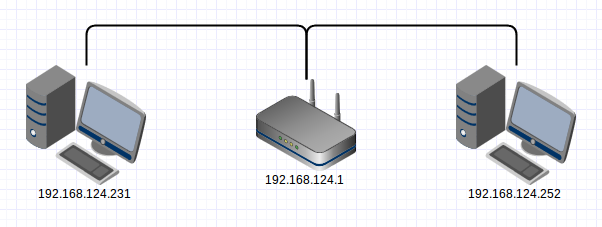
\includegraphics[scale=0.7]{img/01_topology}
\caption{Топология сети.}
\end{figure}

\vspace{1em}
Исходный код всех представленных листингов доступен по адресу \\ \url{https://github.com/SemenMartynov/SPbPU_SystemProgramming}.

\setcounter{page}{2}

\newpage
%------------------------------------------------
\section*{Анонимные каналы}

Анонимные каналы (anonymous channels) Windows обеспечивают однонаправленное (полудуплексное) посимвольное межпроцессное взаимодействие. Каждый канал имеет два дескриптора: дескриптор чтения (read handle) и дескриптор записи (write handle). Функция, с помощью которой создаются анонимные каналы, имеет следующий прототип:

\begin{verbatim}
BOOL CreatePipe(PHANDLE phRead, PHANDLE phWrite,
                                  LPSECURITY_ATTRIBUTES lpsa, DWORD cbPipe)
\end{verbatim}

Дескрипторы каналов часто бывают наследуемыми; причины этого станут понятными из приведенного ниже примера. Значение параметра cbPipe, указывающее размер канала в байтах, носит рекомендательный характер, причем значению 0 соответствует размер канала по умолчанию.

Чтобы канал можно было использовать для IPC, должен существовать еще один процесс, и для этого процесса требуется один из дескрипторов канала. Предположим, например, что родительскому процессу, вызвавшему функцию CreatePipe, необходимо вывести данные, которые нужны дочернему процессу. Тогда возникает вопрос о том, как передать дочернему процессу дескриптор чтения (phRead). Родительский процесс осуществляет это, устанавливая дескриптор стандартного ввода в структуре STARTUPINFO для дочерней процедуры равным *phRead.

Чтение с использованием дескриптора чтения канала блокируется, если канал пуст. В противном случае в процессе чтения будет воспринято столько байтов, сколько имеется в канале, вплоть до количества, указанного при вызове функции ReadFile. Операция записи в заполненный канал, которая выполняется с использованием буфера в памяти, также будет блокирована.

Наконец, анонимные каналы обеспечивают только однонаправленное взаимодействие. Для двухстороннего взаимодействия необходимы два канала.

В листинге 1 Представлен сервер, а в листинге 2 клиент для работы с анонимными каналами Windows. В программе используется передача дескрипторов через наследование. Рисунок 2 показывает результат работы.

\begin{verbatim}
Листинг 1. Реализация сервера для анонимного канала.

#include <windows.h>
#include <stdio.h>
int main(int argc, char* argv[])
{
    //дескрипторы канала для передачи от сервера клиенту
    HANDLE hReadPipeFromServToClient, hWritePipeFromServToClient;
    //дескрипторы канала для передачи от клиента к серверу
    HANDLE hReadPipeFromClientToServ, hWritePipeFromClientToServ;

    //чтобы сделать дескрипторы наследуемыми создаем канал для передачи
    //от сервера клиенту, сразу делаем дескрипторы наследуемыми
    SECURITY_ATTRIBUTES PipeSA = { sizeof(SECURITY_ATTRIBUTES), NULL, TRUE };
    if (CreatePipe(&hReadPipeFromServToClient,
                                &hWritePipeFromServToClient, &PipeSA, 0) == 0)
    {
        printf("impossible to create anonymous pipe from serv to client\n");
        getchar();
        return 1000;
    }
    //создаем канал для передачи от клиента серверу,
    // сразу делаем дескрипторы наследуемыми
    if (CreatePipe(&hReadPipeFromClientToServ,
                                &hWritePipeFromClientToServ, &PipeSA, 0) == 0)
    {
        printf("impossible to create anonymous pipe from client to serv\n");
        getchar();
        return 1001;
    }

    PROCESS_INFORMATION processInfo_Client; // информация о процессе-клиенте
    //структура, которая описывает внешний вид основного окна и содержит
    //дескрипторы стандартных устройств нового процесса, используем для установки
    STARTUPINFOA startupInfo_Client;
    
    //процесс-клиент будет иметь те же параметры запуска, что и сервер,
    //за исключением дескрипторов ввода, вывода и ошибок
    GetStartupInfoA(&startupInfo_Client);
    startupInfo_Client.hStdInput = hReadPipeFromServToClient;
    //устанавливаем поток ввода
    startupInfo_Client.hStdOutput = hWritePipeFromClientToServ;
    //установим поток вывода
    startupInfo_Client.hStdError = GetStdHandle(STD_ERROR_HANDLE);
    //установим поток ошибок
    startupInfo_Client.dwFlags = STARTF_USESTDHANDLES;
    //устанавливаем наследование создаем процесс клиента
    CreateProcessA(NULL, "AnonymousPipeClient.exe", NULL,
        NULL, TRUE, CREATE_NEW_CONSOLE, NULL, NULL,
        &startupInfo_Client, &processInfo_Client);
    //закрываем дескрипторы созданного процесса и его потока
    CloseHandle(processInfo_Client.hThread);
    CloseHandle(processInfo_Client.hProcess);
    //закрываем ненужные дескрипторы каналов, которые не использует сервер
    CloseHandle(hReadPipeFromServToClient);
    CloseHandle(hWritePipeFromClientToServ);
#define BUF_SIZE 100
    //размер буфера для сообщений
    BYTE buf[BUF_SIZE];
    //буфер приема/передачи
    DWORD readbytes, writebytes; //число прочитанных/переданных байт
    for (int i = 0; i < 10; i++)
    {
        //читаем данные из канала от клиента
        if (!ReadFile(hReadPipeFromClientToServ, buf, BUF_SIZE, &readbytes, NULL))
        {
            printf("impossible to use readfile\n GetLastError= %d\n", GetLastError());
            getchar();
            return 10000;
        }
        printf("get from client: \"%s\"\n", buf);
        if (!WriteFile(hWritePipeFromServToClient, buf, readbytes, &writebytes, NULL))
        {
            printf("impossible to use writefile\n GetLastError= %d\n", GetLastError());
            getchar();
            return 10001;
        }
        //пишем данные в канал клиенту
    }
    //закрываем HANDLE каналов
    CloseHandle(hReadPipeFromClientToServ);
    CloseHandle(hWritePipeFromServToClient);
    printf("server ended work\n Press any key");
    getchar();
    return 0;
}
\end{verbatim}

\vspace{3em}

\begin{verbatim}
Листинг 2. Реализация клиента для анонимного канала.

#include <stdio.h>
#include <Windows.h>
int main(int argc, char* argv[])
{
    //строка для передачи
    char strtosend[100];
    //буфер приема
    char getbuf[100];
    //число переданных и принятых байт
    DWORD bytessended, bytesreaded;
    
    for (int i = 0; i < 10; i++)
    {
        //формирование строки для передачи
        bytessended = sprintf_s(strtosend, "message num %d", i + 1);
        strtosend[bytessended] = 0;
        fprintf(stderr, "client sended: \"%s\"\n", strtosend);
        if (!WriteFile(GetStdHandle(STD_OUTPUT_HANDLE), strtosend,
                                            bytessended + 1, &bytesreaded, NULL)
            ) //передача данных
        {
            fprintf(stderr, 
                "Error with writeFile\n Wait 5 sec GetLastError=%d\n",
                GetLastError());
            Sleep(5000);
            return 1000;
        }
        if (!ReadFile(GetStdHandle(STD_INPUT_HANDLE),
                                               getbuf, 100, &bytesreaded, NULL))
            //прием ответа от сервера
        {
            fprintf(stderr,
                "Error with readFile\n Wait 5 sec GetLastError=%d\n",
                 GetLastError());
            Sleep(5000);
            return 1001;
        }
        fprintf(stderr, "Get msg from server: \"%s\"\n", getbuf);
    }
    fprintf(stderr, "client ended work\n");
    getchar();
    return 0;
}
\end{verbatim}

\begin{figure}[h!]
\centering
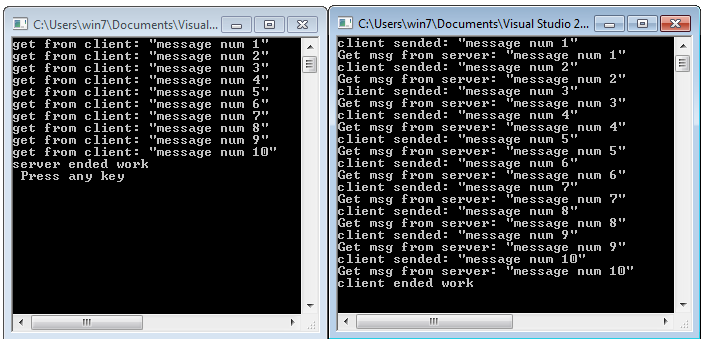
\includegraphics[scale=0.95]{img/02_anonymous_channels}
\caption{Работа с анонимными каналами.}
\end{figure}

\newpage
%------------------------------------------------
\section*{Именованные каналы}

Именованные каналы (named pipes) предлагают ряд возможностей, которые делают их полезными в качестве универсального механизма реализации приложений на основе IPC, включая приложения, требующие сетевого доступа к файлам, и клиент-серверные системы, хотя для реализации простых вариантов IPC, ориентированных на байтовые потоки, как в предыдущем примере, в котором взаимодействие процессов ограничивается рамками одной системы, анонимных каналов вам будет вполне достаточно. К числу упомянутых возможностей (часть которых обеспечивается дополнительно) относятся следующие:

\begin{itemize}
\item Именованные каналы ориентированы на обмен сообщениями, поэтому процесс, выполняющий чтение, может считывать сообщения переменной длины именно в том виде, в каком они были посланы процессом, выполняющим запись.

\item Именованные каналы являются двунаправленными, что позволяет осуществлять обмен сообщениями между двумя процессами посредством единственного канала.

\item Допускается существование нескольких независимых экземпляров канала, имеющих одинаковые имена. Например, с единственной серверной системой могут связываться одновременно несколько клиентов, использующих каналы с одним и тем же именем. Каждый клиент может иметь собственный экземпляр именованного канала, и сервер может использовать этот же канал для отправки ответа клиенту.

\item Каждая из систем, подключенных к сети, может обратиться к каналу, используя его имя. Взаимодействие посредством именованного канала осуществляется одинаковым образом для процессов, выполняющихся как на одной и той же, так и на разных машинах.

\item Имеется несколько вспомогательных и связных функций, упрощающих обслуживание взаимодействия "запрос/ответ" и клиент-серверных соединений.
\end{itemize}

Как правило, именованные каналы являются более предпочтительными по сравнению с анонимными, хотя существуют ситуации, когда анонимные каналы оказываются исключительно полезными. Во всех случаях, когда требуется, чтобы канал связи был двунаправленным, ориентированным на обмен сообщениями или доступным для нескольких клиентских процессов, следует применять именованные каналы. Попытки реализации последующих примеров с использованием анонимных каналов натолкнулись бы на значительные трудности.

Листинг 3 содержит код, реализующий сервер именованного канала. В листинге 4 - код клиента. Рисунок 3 - результат работы одного сервера с несколькими клиентами. Сервер не содержит разделяемых ресурсов, следовательно в средствах синхронизации потоков необходимости нет.

\begin{verbatim}
Листинг 3. Реализация сервера для именованного канала.

//http://msdn.microsoft.com/ru-ru/windows/desktop/aa365802%28v=vs.85%29

#include <windows.h> 
#include <stdio.h> 
#include <conio.h>
#include <tchar.h>
#include <strsafe.h>

#define BUFSIZE 512

DWORD WINAPI InstanceThread(LPVOID);

int _tmain(int argc, TCHAR *argv[])
{
    _tprintf(TEXT("Server is started.\n\n"));

    BOOL   fConnected = FALSE; // Флаг наличия подключенных клиентов
    DWORD  dwThreadId = 0; // Номер обслуживающего потока
    HANDLE hPipe = INVALID_HANDLE_VALUE; // Идентификатор канала
    HANDLE hThread = NULL; // Идентификатор обслуживающего потока
    // Имя создаваемого канала Pipe
    LPTSTR lpszPipename = TEXT("\\\\.\\pipe\\$$MyPipe$$");

    // Цикл ожидает клиентов и создаёт для них потоки обработки
    for (;;)
    {
        _tprintf(TEXT("Try to create named pipe on %s\n"), lpszPipename);

        // Создаем канал:
        hPipe = CreateNamedPipe(
            // имя канала,
            lpszPipename,
            // режим открытия канала - двунаправленный,
            PIPE_ACCESS_DUPLEX,
            // данные записываются в канал в виде потока сообщений,
            PIPE_TYPE_MESSAGE |
            // данные считываются в виде потока сообщений,
            PIPE_READMODE_MESSAGE |
            // функции передачи и приема блокируются до их окончания,
            PIPE_WAIT,
            // максимальное число экземпляров каналов не ограничено,
            PIPE_UNLIMITED_INSTANCES,
            //размеры выходного и входного буферов канала,
            BUFSIZE,
            BUFSIZE,
            // 5 секунд - длительность для функции WaitNamedPipe,
            5000,
            // дескриптор безопасности по умолчанию.
            NULL);

        // Если возникла ошибка, выводим ее код и завершаем работу приложения
        if (hPipe == INVALID_HANDLE_VALUE)
        {
            _tprintf(TEXT("CreateNamedPipe failed, GLE=%d.\n"), GetLastError());
            _getch();
            return -1;
        }
        _tprintf(TEXT("Named pipe created successfully!\n\n"));

        // Ожидаем соединения со стороны клиента
        _tprintf(TEXT("Waiting for connect...\n"));
        fConnected = ConnectNamedPipe(hPipe, NULL) ?
            TRUE :
            (GetLastError() == ERROR_PIPE_CONNECTED);

        // Если произошло соединение
        if (fConnected)
        {
            _tprintf(TEXT("Client connected!\n\nCreating a processing thread...\n"));

            // Создаём поток для обслуживания клиента 
            hThread = CreateThread(
                NULL,              // дескриптор защиты 
                0,                 // начальный размер стека
                InstanceThread,    // функция потока
                (LPVOID)hPipe,     // параметр потока
                0,                 // опции создания
                &dwThreadId);      // номер потока

            // Если поток создать не удалось - сообщаем об ошибке
            if (hThread == NULL)
            {
                _tprintf(TEXT("CreateThread failed, GLE=%d.\n"), GetLastError());
                _getch();
                return -1;
            }
            else CloseHandle(hThread);
        }
        else
            // Если клиенту не удалось подключиться, закрываем канал
            CloseHandle(hPipe);
    }

    return 0;
}

DWORD WINAPI InstanceThread(LPVOID lpvParam)
{
    _tprintf(TEXT("Thread started!\n"));
    HANDLE hPipe = (HANDLE)lpvParam; // Идентификатор канала
    // Буфер для хранения полученного и передаваемого сообщения
    TCHAR* chBuf = (TCHAR*)HeapAlloc(GetProcessHeap(), 0, BUFSIZE * sizeof(TCHAR));
    DWORD readbytes, writebytes; // Число байт прочитанных и переданных

    while (1)
    {
        // Получаем очередную команду через канал Pipe
        if (ReadFile(hPipe, chBuf, BUFSIZE*sizeof(TCHAR), &readbytes, NULL))
        {
            // Посылаем эту команду обратно клиентскому приложению
            if (!WriteFile(hPipe, chBuf, (lstrlen(chBuf) + 1)*sizeof(TCHAR),
                                                            &writebytes, NULL))
                break;
            // Выводим принятую команду на консоль
            _tprintf(TEXT("Get client msg: %s\n"), chBuf);
            // Если пришла команда "exit", завершаем работу приложения
            if (!_tcsncmp(chBuf, L"exit", 4))
                break;
        }
        else
        {
            _tprintf(TEXT("ReadFile: Error %ld\n"), GetLastError());
            _getch();
            break;
        }
    }

    // Освобождение ресурсов 
    FlushFileBuffers(hPipe);
    DisconnectNamedPipe(hPipe);
    CloseHandle(hPipe);
    HeapFree(hPipe, 0, chBuf);

    _tprintf(TEXT("InstanceThread exitting.\n"));
    return 1;
}
\end{verbatim}

\vspace{3em}

\begin{verbatim}
Листинг 4. Код клиента именованного канала.

//http://msdn.microsoft.com/ru-ru/windows/desktop/aa365785%28v=vs.85%29

#include <windows.h> 
#include <stdio.h>
#include <conio.h>
#include <tchar.h>
#include <strsafe.h>

#define BUFSIZE 512

int _tmain(int argc, TCHAR *argv[])
{
    _tprintf(TEXT("Client is started!\n\n"));

    HANDLE hPipe = INVALID_HANDLE_VALUE; // Идентификатор канала
    // Имя создаваемого канала Pipe
    LPTSTR lpszPipename = TEXT("\\\\.\\pipe\\$$MyPipe$$");
    TCHAR chBuf[BUFSIZE]; // Буфер для передачи данных через канал
    DWORD readbytes, writebytes; // Число байт прочитанных и переданных

    _tprintf(TEXT("Try to use WaitNamedPipe...\n"));
    // Пытаемся открыть именованный канал, если надо - ожидаем его освобождения
    while (1)
    {
        // Создаем канал с процессом-сервером:
        hPipe = CreateFile(
            lpszPipename, // имя канала,
            GENERIC_READ // текущий клиент имеет доступ на чтение,
            | GENERIC_WRITE, // текущий клиент имеет доступ на запись,
            0, // тип доступа,
            NULL, // атрибуты защиты,
            OPEN_EXISTING, // открывается существующий файл,
            0, // атрибуты и флаги для файла,
            NULL); // доступа к файлу шаблона.

        // Продолжаем работу, если канал создать удалось 
        if (hPipe != INVALID_HANDLE_VALUE)
            break;

        // Выход, если ошибка связана не с занятым каналом. 
        if (GetLastError() != ERROR_PIPE_BUSY)
        {
            _tprintf(TEXT("Could not open pipe. GLE=%d\n"), GetLastError());
            _getch();
            return -1;
        }

        // Если все каналы заняты, ждём 20 секунд 
        if (!WaitNamedPipe(lpszPipename, 20000))
        {
            _tprintf(TEXT("Could not open pipe: 20 second wait timed out."));
            _getch();
            return -1;
        }
    }

    // Выводим сообщение о создании канала
    _tprintf(TEXT("Successfully connected!\n\nInput message...\n"));
    // Цикл обмена данными с серверным процессом
    while (1)
    {
        // Выводим приглашение для ввода команды
        _tprintf(TEXT("cmd>"));
        // Вводим текстовую строку
        _fgetts(chBuf, BUFSIZE, stdin);
        // Передаем введенную строку серверному процессу в качестве команды
        if (!WriteFile(hPipe, chBuf, (lstrlen(chBuf) + 1)*sizeof(TCHAR),
                                                        &writebytes, NULL))
        {
            _tprintf(TEXT("connection refused\n"));
            break;
        }
        // Получаем эту же команду обратно от сервера
        if (ReadFile(hPipe, chBuf, BUFSIZE*sizeof(TCHAR), &readbytes, NULL))
            _tprintf(TEXT("Received from server: %s\n"), chBuf);
        // Если произошла ошибка, выводим ее код и завершаем работу приложения
        else {
            _tprintf(TEXT("ReadFile: Error %ld\n"), GetLastError());
            _getch();
            break;
        }
        // В ответ на команду "exit" завершаем цикл
        // обмена данными с серверным процессом
        if (!_tcsncmp(chBuf, L"exit", 4))
            break;
    }

    // Закрываем идентификатор канала
    CloseHandle(hPipe);
    
    _tprintf(TEXT("Press ENTER to terminate connection and exit\n"));
    _getch();
    return 0;
}
\end{verbatim}

\begin{figure}[h!]
\centering
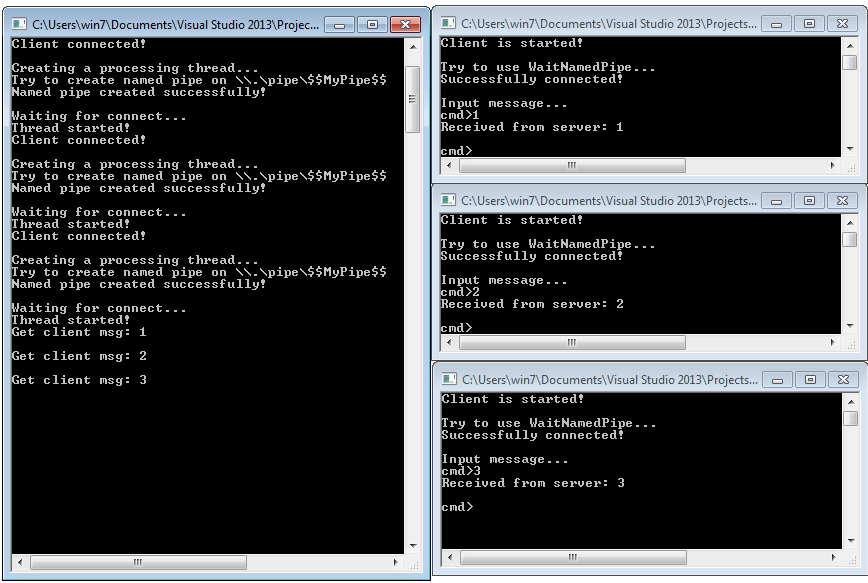
\includegraphics[scale=0.8]{img/03_named_pipes}
\caption{Работа с нескольких клиентов с одним сервером по именованному каналу.}
\end{figure}

Помимо локального обмена, именованные каналы могут использоваться и для сетевого взаимодействия. Это требует не большой доработки клиента в части указания пути к каналу и изменения настроек безопасности. В листинге 5 содержится отрывок кода клиента с самыми значительными изменениями. Результаты работы внешне не отличаются от работы в локальном варианте.

\begin{verbatim}
Листинг 5. Отрывок кода клиента, работающего с именованным каналом по сети.

+++
    _tprintf(TEXT("Client is started!\n\n"));

    HANDLE hPipe = INVALID_HANDLE_VALUE; // Идентификатор канала
     // Имя создаваемого канала Pipe
    LPTSTR lpszPipename = TEXT("\\\\192.168.124.2\\pipe\\$$MyPipe$$");
    TCHAR chBuf[BUFSIZE]; // Буфер для передачи данных через канал
    DWORD readbytes, writebytes; // Число байт прочитанных и переданных

    // Создание SECURITY_ATTRIBUTES и SECURITY_DESCRIPTOR объектов
    SECURITY_ATTRIBUTES sa;
    SECURITY_DESCRIPTOR sd;
    // Инициализация SECURITY_DESCRIPTOR значениями по-умолчанию
    if (InitializeSecurityDescriptor(&sd, SECURITY_DESCRIPTOR_REVISION) == 0)
    {
        _tprintf(TEXT("InitializeSecurityDescriptor failed with error %d\n"),
                                                                GetLastError());
        _getch();
        return -1;
    }
    // Установка поля DACL в SECURITY_DESCRIPTOR в NULL
    if (SetSecurityDescriptorDacl(&sd, TRUE, NULL, FALSE) == 0)
    {
        _tprintf(TEXT("SetSecurityDescriptorDacl failed with error %d\n"),
                                                                GetLastError());
        _getch();
        return -1;
    }
    // Установка SECURITY_DESCRIPTOR в структуре SECURITY_ATTRIBUTES
    sa.nLength = sizeof(SECURITY_ATTRIBUTES);
    sa.lpSecurityDescriptor = &sd;
    sa.bInheritHandle = FALSE; //запрещение наследования

    _tprintf(TEXT("Try to use WaitNamedPipe...\n"));
    // Пытаемся открыть именованный канал, если надо - ожидаем его освобождения
    while (1)
    {
        // Создаем канал с процессом-сервером:
        hPipe = CreateFile(
            lpszPipename, // имя канала,
            GENERIC_READ // текущий клиент имеет доступ на чтение,
            | GENERIC_WRITE, // текущий клиент имеет доступ на запись,
            0, // тип доступа,
            &sa, // атрибуты защиты,
            OPEN_EXISTING, // открывается существующий файл,
            0, // атрибуты и флаги для файла,
            NULL); // доступа к файлу шаблона.

+++
\end{verbatim}

\newpage
%------------------------------------------------
\section*{Почтовые ящики}

Как и именованные каналы, почтовые ящики (mailslots) Windows снабжаются именами, которые могут быть использованы для обеспечения взаимодействия между независимыми каналами. Почтовые ящики представляют собой широковещательный механизм, и ведут себя иначе по сравнению с именованными каналами, что делает их весьма полезными в ряде ограниченных ситуаций, которые, тем не менее, представляют большой интерес. Из наиболее важных свойств почтовых ящиков можно отметить следующие:

\begin{itemize}
\item Почтовые ящики являются однонаправленными.

\item С одним почтовым ящиком могут быть связаны несколько записывающих программ (writers) и несколько считывающих программ (readers), но они часто связаны между собой отношениями "один ко многим" в той или иной форме.

\item Записывающей программе (клиенту) не известно достоверно, все ли, только некоторые или какая-то одна из программ считывания (сервер) получили сообщение.

\item Почтовые ящики могут находиться в любом месте сети.

\item Размер сообщений ограничен.
\end{itemize}

Использование почтовых ящиков требует выполнения следующих операций:
\begin{itemize}
\item Каждый сервер создает дескриптор почтового ящика с помощью функции CreateMailSlot.

\item После этого сервер ожидает получения почтового сообщения, используя функцию ReadFile.

\item Клиент, обладающий только правами записи, должен открыть почтовый ящик, вызвав функцию CreateFile, и записать сообщения, используя функцию WriteFile. В случае отсутствия ожидающих программ считывания попытка открытия почтового ящика завершится ошибкой (наподобие "имя не найдено").
\end{itemize}

Сообщение клиента может быть прочитано всеми серверами; все серверы получают одно и то же сообщение.

Существует еще одна возможность. В вызове функции CreateFile клиент может указать имя почтового ящика в следующем виде:

\begin{verbatim}
\\*\mailslot\mailslotname
\end{verbatim}

При этом символ звездочки (*) действует в качестве группового символа (wildcard), и клиент может обнаружить любой сервер в пределах имени домена — группы систем, объединенных общим именем, которое назначается администратором сети. 

Листинг 6 и 7 демонстрируют реализацию приложения, иллюстрирующую обмен информацией почтовыми слотами. В процессе экспериментов было протестировано локальное, сетевое взаимодействие. Для широковещательной передач сообщений, адрес заменялся символом звездочки (*).

\begin{verbatim}
Листинг 6. Реализация серверной части почтового ящика.

//http://msdn.microsoft.com/ru-ru/windows/desktop/aa365802%28v=vs.85%29

#include <windows.h>
#include <stdio.h>
#include <conio.h>

LPTSTR SlotName = TEXT("\\\\.\\mailslot\\sample_mailslot");

BOOL WriteSlot(HANDLE hSlot, LPTSTR lpszMessage)
{
    BOOL fResult;
    DWORD cbWritten;

    fResult = WriteFile(hSlot,
        lpszMessage,
        (DWORD)(lstrlen(lpszMessage) + 1)*sizeof(TCHAR),
        &cbWritten,
        (LPOVERLAPPED)NULL);

    if (!fResult)
    {
        printf("WriteFile failed with %d.\n", GetLastError());
        return FALSE;
    }

    printf("Slot written to successfully.\n");

    return TRUE;
}

int main()
{
    HANDLE hFile;

    hFile = CreateFile(SlotName,
        GENERIC_WRITE,
        FILE_SHARE_READ,
        (LPSECURITY_ATTRIBUTES)NULL,
        OPEN_EXISTING,
        FILE_ATTRIBUTE_NORMAL,
        (HANDLE)NULL);

    if (hFile == INVALID_HANDLE_VALUE)
    {
        printf("CreateFile failed with %d.\n", GetLastError());
        return FALSE;
    }

    WriteSlot(hFile, TEXT("Message one for mailslot."));
    WriteSlot(hFile, TEXT("Message two for mailslot."));
    Sleep(5000);
    WriteSlot(hFile, TEXT("Message three for mailslot."));
    CloseHandle(hFile);
    _getch();
    return TRUE;
}
\end{verbatim}

\vspace{3em}

\begin{verbatim}
Листинг 7. Реализация клиентской части почтового ящика.

//http://msdn.microsoft.com/ru-ru/windows/desktop/aa365785%28v=vs.85%29

#include <windows.h>
#include <tchar.h>
#include <stdio.h>
#include <strsafe.h>
#include <conio.h>

HANDLE hSlot;
LPTSTR SlotName = TEXT("\\\\.\\mailslot\\sample_mailslot");

BOOL ReadSlot()
{
    DWORD cbMessage, cMessage, cbRead;
    BOOL fResult;
    LPTSTR lpszBuffer;
    TCHAR achID[80];
    DWORD cAllMessages;
    HANDLE hEvent;
    OVERLAPPED ov;

    cbMessage = cMessage = cbRead = 0;

    hEvent = CreateEvent(NULL, FALSE, FALSE, TEXT("ExampleSlot"));
    if (NULL == hEvent)
        return FALSE;
    ov.Offset = 0;
    ov.OffsetHigh = 0;
    ov.hEvent = hEvent;

    fResult = GetMailslotInfo(hSlot, // mailslot handle 
        (LPDWORD)NULL,               // no maximum message size 
        &cbMessage,                   // size of next message 
        &cMessage,                    // number of messages 
        (LPDWORD)NULL);              // no read time-out 

    if (!fResult)
    {
        printf("GetMailslotInfo failed with %d.\n", GetLastError());
        return FALSE;
    }

    if (cbMessage == MAILSLOT_NO_MESSAGE)
    {
        printf("Waiting for a message...\n");
        return TRUE;
    }

    cAllMessages = cMessage;

    while (cMessage != 0)  // retrieve all messages
    {
        // Create a message-number string. 

        StringCchPrintf((LPTSTR)achID,
            80,
            TEXT("\nMessage #%d of %d\n"),
            cAllMessages - cMessage + 1,
            cAllMessages);

        // Allocate memory for the message. 

        lpszBuffer = (LPTSTR)GlobalAlloc(GPTR,
            lstrlen((LPTSTR)achID)*sizeof(TCHAR) + cbMessage);
        if (NULL == lpszBuffer)
            return FALSE;
        lpszBuffer[0] = '\0';

        fResult = ReadFile(hSlot,
            lpszBuffer,
            cbMessage,
            &cbRead,
            &ov);

        if (!fResult)
        {
            printf("ReadFile failed with %d.\n", GetLastError());
            GlobalFree((HGLOBAL)lpszBuffer);
            return FALSE;
        }

        // Concatenate the message and the message-number string. 

        StringCbCat(lpszBuffer,
            lstrlen((LPTSTR)achID)*sizeof(TCHAR) + cbMessage,
            (LPTSTR)achID);

        // Display the message. 

        _tprintf(TEXT("Contents of the mailslot: %s\n"), lpszBuffer);

        GlobalFree((HGLOBAL)lpszBuffer);

        fResult = GetMailslotInfo(hSlot,  // mailslot handle 
            (LPDWORD)NULL,               // no maximum message size 
            &cbMessage,                   // size of next message 
            &cMessage,                    // number of messages 
            (LPDWORD)NULL);              // no read time-out 

        if (!fResult)
        {
            printf("GetMailslotInfo failed (%d)\n", GetLastError());
            return FALSE;
        }
    }
    CloseHandle(hEvent);
    return TRUE;
}

BOOL WINAPI MakeSlot(LPTSTR lpszSlotName)
{
    hSlot = CreateMailslot(lpszSlotName,
        0,                             // no maximum message size 
        MAILSLOT_WAIT_FOREVER,         // no time-out for operations 
        (LPSECURITY_ATTRIBUTES)NULL); // default security

    if (hSlot == INVALID_HANDLE_VALUE)
    {
        printf("CreateMailslot failed with %d\n", GetLastError());
        return FALSE;
    }
    return TRUE;
}

void main()
{
    MakeSlot(SlotName);

    while (TRUE)
    {
        ReadSlot();
        Sleep(3000);
    }
    _getch();
}

\end{verbatim}

\begin{figure}[h!]
\centering
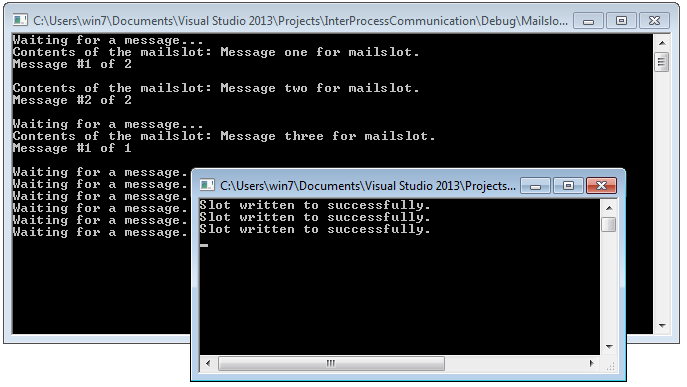
\includegraphics[scale=0.95]{img/04_MailSlot}
\caption{Работа почтовыми ящиками.}
\end{figure}

\newpage
%------------------------------------------------
\section*{Shared memory}

Этот способ взаимодействия реализуется через технологию File Mapping - отображения файлов на оперативную память. Механизм позволяет осуществлять доступ к файлу таким образом, как будто это обыкновенный массив, хранящийся в памяти (не загружая файл в память явно). Можно создать объект file mapping, но не ассоциировать его с каким-то конкретным файлом. Получаемая область памяти будет общей между процессами. Работая с этой памятью, потоки обязательно должны согласовывать свои действия с помощью объектов синхронизации.

В листинге 8 и 9 представлен код двух программ, одна из которых генерирует случайные числа, а другая их читает и выводит на экран. Взаимодействие осуществляется через разделяемую память, защищённую мьютексом. Рисунок 5 показывает результат такого взаимодействия.

\begin{verbatim}
Листинг 8. Программа, генерирующая случайные числа в разделяемую память.

#include <windows.h>
#include <stdio.h>
#include <conio.h>
#define BUF_SIZE 256
TCHAR szName[] = TEXT("MyFileMappingObject");
TCHAR szMsg[] = TEXT("Message from first process");
HANDLE mutex;
void main()
{
    HANDLE hMapFile;
    LPCTSTR pBuf;
    mutex = CreateMutex(NULL, false, TEXT("SyncMutex"));
    // create a memory, wicth two proccess will be working
    hMapFile = CreateFileMapping(
        // использование файла подкачки
        INVALID_HANDLE_VALUE,
        // защита по умолчанию
        NULL,
        // доступ к чтению/записи
        PAGE_READWRITE,
        // макс. размер объекта
        0,
        // размер буфера
        BUF_SIZE,
        // имя отраженного в памяти объекта
        szName);

    if (hMapFile == NULL || hMapFile == INVALID_HANDLE_VALUE)
    {
        printf("Не может создать отраженный в памяти объект (%d).\n",
            GetLastError());
        return;
    }
    pBuf = (LPTSTR)MapViewOfFile(
        //дескриптор проецируемого в памяти объекта
        hMapFile,
        // разрешение чтения/записи(режим доступа)
        FILE_MAP_ALL_ACCESS,
        //Старшее слово смещения файла, где начинается отображение
        0,
        //Младшее слово смещения файла, где начинается отображение
        0,
        //Число отображаемых байтов файла
        BUF_SIZE);
    
    if (pBuf == NULL)
    {
        printf("Представление проецированного файла невозможно (%d).\n",
            GetLastError());
        return;
    }

    int i = 0;
    while (true)
    {
        i = rand();
        itoa(i, (char *)szMsg, 10);
        WaitForSingleObject(mutex, INFINITE);
        CopyMemory((PVOID)pBuf, szMsg, sizeof(szMsg));
        printf("write message: %s\n", (char *)pBuf);
        //необходимо только для отладки - для удобства представления и анализа
        Sleep(1000);
        //результатов
        ReleaseMutex(mutex);
    }
    // освобождение памяти и закрытие описателя handle
    UnmapViewOfFile(pBuf);
    CloseHandle(hMapFile);
    CloseHandle(mutex);
}
\end{verbatim}

\vspace{3em}

\begin{verbatim}
Листинг 9. Программа, читающая случайные числа из разделяемой памяти.

#include <windows.h>
#include <stdio.h>
#include <conio.h>
#define BUF_SIZE 256
#define TIME 15
// number of reading operation in this process
TCHAR szName[] = TEXT("MyFileMappingObject");
HANDLE mutex;
void main()
{
    HANDLE hMapFile;
    LPCTSTR pBuf;
    mutex = OpenMutex(
        // request full access
        MUTEX_ALL_ACCESS,
        // handle not inheritable
        FALSE,
        // object name
        TEXT("SyncMutex"));
    if (mutex == NULL)
        printf("OpenMutex error: %d\n", GetLastError());
    else printf("OpenMutex successfully opened the mutex.\n");
    hMapFile = OpenFileMapping(
        // доступ к чтению/записи
        FILE_MAP_ALL_ACCESS,
        // имя не наследуется
        FALSE,
        // имя "проецируемого " объекта
        szName);
    if (hMapFile == NULL)
    {
        printf("Невозможно открыть объект проекция файла (%d).\n", GetLastError());
        return;
    }
    pBuf = (LPTSTR)MapViewOfFile(hMapFile,
        // дескриптор "проецируемого" объекта
        FILE_MAP_ALL_ACCESS, // разрешение чтения/записи
        0,
        0,
        BUF_SIZE);
    if (pBuf == NULL)
    {
        printf("Представление проецированного файла (%d) невозможно .\n",
            GetLastError());
        return;
    }
    for (int i = 0; i < TIME; i++)
    {
        WaitForSingleObject(mutex, INFINITE);
        printf("read message: %s\n", (char *)pBuf);
        ReleaseMutex(mutex);
    }
    UnmapViewOfFile(pBuf);
    CloseHandle(hMapFile);
}

\end{verbatim}

\begin{figure}[h!]
\centering
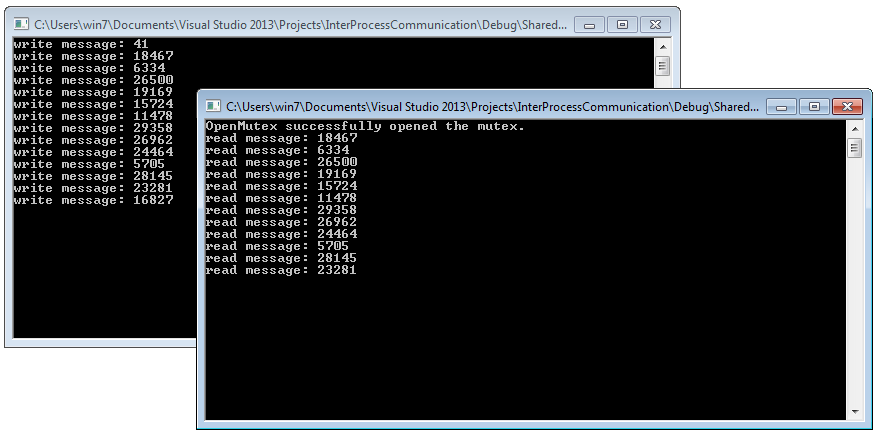
\includegraphics[scale=0.8]{img/05_Sharedmemory}
\caption{Работа с разделяемой памятью.}
\end{figure}

\newpage
%------------------------------------------------
\section*{Сокеты}

Winsock API разрабатывался как расширение Berkley Sockets API для среды Windows и поэтому поддерживается всеми системами Windows. К преимуществам Winsock можно отнести следующее:

\begin{itemize}
\item Перенос уже имеющегося кода, написанного для Berkeley Sockets API, осуществляется непосредственно.

\item Системы Windows легко встраиваются в сети, использующие как версию IPv4 протокола TCP/IP, так и постепенно распространяющуюся версию IPv6. Помимо всего остального, версия IPv6 допускает использование более длинных IP-адресов, преодолевая существующий 4-байтовый адресный барьер версии IPv4.

\item Сокеты могут использоваться совместно с перекрывающимся вводом/выводом Windows (глава 14), что, помимо всего прочего, обеспечивает возможность масштабирования серверов при увеличении количества активных клиентов.

\item Сокеты можно рассматривать как дескрипторы (типа HANDLE) файлов при использовании функций ReadFile и WriteFile и, с некоторыми ограничениями, при использовании других функций, точно так же, как в качестве дескрипторов файлов сокеты применяются в UNIX. Эта возможность оказывается удобной в тех случаях, когда требуется использование асинхронного ввода/вывода и портов завершения ввода/вывода.

\item Существуют также дополнительные, непереносимые расширения.
\end{itemize}

Работа с сокетами демонстрируется в листинге 10 и 11. Рисунок 6 показывает работу программ, из этих листингов.

\begin{verbatim}
Листинг 10. Сервер для работы с Win-сокетами.

// http://navendus.tripod.com

#define _WINSOCK_DEPRECATED_NO_WARNINGS
#include <winsock2.h>
#include <iostream>

#pragma comment(lib, "Ws2_32.lib")

struct CLIENT_INFO
{
    SOCKET hClientSocket;
    struct sockaddr_in clientAddr;
};

char szServerIPAddr[] = "127.0.0.1"; // server IP
int nServerPort = 5050;  // server port
// clients to talk with the server

bool InitWinSock2_0();
BOOL WINAPI ClientThread(LPVOID lpData);

int main()
{
    if (!InitWinSock2_0())
    {
        std::cout << "Unable to Initialize Windows Socket environment"
            << WSAGetLastError() << std::endl;
        return -1;
    }

    SOCKET hServerSocket;

    hServerSocket = socket(
        AF_INET,        // The address family. AF_INET specifies TCP/IP
        SOCK_STREAM,    // Protocol type. SOCK_STREM specified TCP
        0               // Protoco Name. Should be 0 for AF_INET address family
        );
    if (hServerSocket == INVALID_SOCKET)
    {
        std::cout << "Unable to create Server socket" << std::endl;
        // Cleanup the environment initialized by WSAStartup()
        WSACleanup();
        return -1;
    }

    // Create the structure describing various Server parameters
    struct sockaddr_in serverAddr;

    serverAddr.sin_family = AF_INET;     // The address family. MUST be AF_INET
    serverAddr.sin_addr.s_addr = inet_addr(szServerIPAddr);
    serverAddr.sin_port = htons(nServerPort);

    // Bind the Server socket to the address & port
    if (bind(hServerSocket, (struct sockaddr *) &serverAddr,
                                            sizeof(serverAddr)) == SOCKET_ERROR)
    {
        std::cout << "Unable to bind to " << szServerIPAddr
                                        << " port " << nServerPort << std::endl;
        // Free the socket and cleanup the environment initialized by WSAStartup()
        closesocket(hServerSocket);
        WSACleanup();
        return -1;
    }

    // Put the Server socket in listen state
    // so that it can wait for client connections
    if (listen(hServerSocket, SOMAXCONN) == SOCKET_ERROR)
    {
        std::cout << "Unable to put server in listen state" << std::endl;
        // Free the socket and cleanup the
        // environment initialized by WSAStartup()
        closesocket(hServerSocket);
        WSACleanup();
        return -1;
    }

    // Start the infinite loop
    while (true)
    {
        // As the socket is in listen mode there is a connection request pending.
        // Calling accept( ) will succeed and return the socket for the request.
        SOCKET hClientSocket;
        struct sockaddr_in clientAddr;
        int nSize = sizeof(clientAddr);

        hClientSocket = accept(hServerSocket,
                                    (struct sockaddr *) &clientAddr, &nSize);
        if (hClientSocket == INVALID_SOCKET)
        {
            std::cout << "accept( ) failed" << std::endl;
        }
        else
        {
            HANDLE hClientThread;
            struct CLIENT_INFO clientInfo;
            DWORD dwThreadId;

            clientInfo.clientAddr = clientAddr;
            clientInfo.hClientSocket = hClientSocket;

            std::cout << "Client connected from "
                                << inet_ntoa(clientAddr.sin_addr) << std::endl;

            // Start the client thread
            hClientThread = CreateThread(NULL, 0,
                (LPTHREAD_START_ROUTINE)ClientThread,
                (LPVOID)&clientInfo, 0, &dwThreadId);
            if (hClientThread == NULL)
            {
                std::cout << "Unable to create client thread" << std::endl;
            }
            else
            {
                CloseHandle(hClientThread);
            }
        }
    }

    closesocket(hServerSocket);
    WSACleanup();
    return 0;
}

bool InitWinSock2_0()
{
    WSADATA wsaData;
    WORD wVersion = MAKEWORD(2, 0);

    if (!WSAStartup(wVersion, &wsaData))
        return true;

    return false;
}

BOOL WINAPI ClientThread(LPVOID lpData)
{
    CLIENT_INFO *pClientInfo = (CLIENT_INFO *)lpData;
    char szBuffer[1024];
    int nLength;

    while (1)
    {
        nLength = recv(pClientInfo->hClientSocket, szBuffer, sizeof(szBuffer), 0);
        if (nLength > 0)
        {
            szBuffer[nLength] = '\0';
            std::cout << "Received " << szBuffer << " from "
                        << inet_ntoa(pClientInfo->clientAddr.sin_addr) << std::endl;

            // Convert the string to upper case and send it back, if its not QUIT
            _strdup(szBuffer);
            if (strcmp(szBuffer, "QUIT") == 0)
            {
                closesocket(pClientInfo->hClientSocket);
                return TRUE;
            }
            // send( ) may not be able to send the complete data in one go.
            // So try sending the data in multiple requests
            int nCntSend = 0;
            char *pBuffer = szBuffer;

            while ((nCntSend = send(pClientInfo->hClientSocket,
                                                pBuffer, nLength, 0) != nLength))
            {
                if (nCntSend == -1)
                {
                    std::cout << "Error sending the data to "
                    << inet_ntoa(pClientInfo->clientAddr.sin_addr) << std::endl;
                    break;
                }
                if (nCntSend == nLength)
                    break;

                pBuffer += nCntSend;
                nLength -= nCntSend;
            }
        }
        else
        {
            std::cout << "Error reading the data from "
                << inet_ntoa(pClientInfo->clientAddr.sin_addr) << std::endl;
        }
    }

    return TRUE;
}
\end{verbatim}

\vspace{3em}

\begin{verbatim}
Листинг 11. Клиент для работы с Win-сокетами.

#define _WINSOCK_DEPRECATED_NO_WARNINGS
#include <winsock2.h>
#include <iostream>

#pragma comment(lib, "Ws2_32.lib")

char szServerIPAddr[20]; // server IP
int nServerPort; // server port

bool InitWinSock2_0();

int main()
{
    std::cout << "Enter the server IP Address: ";
    std::cin >> szServerIPAddr;
    std::cout << "Enter the server port number: ";
    std::cin >> nServerPort;

    if (!InitWinSock2_0())
    {
        std::cout << "Unable to Initialize Windows Socket environment"
                                            << WSAGetLastError() << std::endl;
        return -1;
    }

    SOCKET hClientSocket;

    hClientSocket = socket(
        AF_INET,        // The address family. AF_INET specifies TCP/IP
        SOCK_STREAM,    // Protocol type. SOCK_STREM specified TCP
        0               // Protoco Name. Should be 0 for AF_INET address family
        );
    if (hClientSocket == INVALID_SOCKET)
    {
        std::cout << "Unable to create Server socket" << std::endl;
        // Cleanup the environment initialized by WSAStartup()
        WSACleanup();
        return -1;
    }


    // Create the structure describing various Server parameters
    struct sockaddr_in serverAddr;

    serverAddr.sin_family = AF_INET;     // The address family. MUST be AF_INET
    serverAddr.sin_addr.s_addr = inet_addr(szServerIPAddr);
    serverAddr.sin_port = htons(nServerPort);

    // Connect to the server
    if (connect(hClientSocket, (struct sockaddr *) &serverAddr,
                                                        sizeof(serverAddr)) < 0)
    {
        std::cout << "Unable to connect to " << szServerIPAddr
                                        << " on port " << nServerPort << std::endl;
        closesocket(hClientSocket);
        WSACleanup();
        return -1;
    }

    char szBuffer[1024] = "";

    while (strcmp(szBuffer, "QUIT") != 0)
    {
        std::cout << "Enter the string to send (QUIT) to stop: ";
        std::cin >> szBuffer;

        int nLength = strlen(szBuffer);

        // send( ) may not be able to send the complete data in one go.
        // So try sending the data in multiple requests
        int nCntSend = 0;
        char *pBuffer = szBuffer;

        while ((nCntSend = send(hClientSocket, pBuffer, nLength, 0) != nLength))
        {
            if (nCntSend == -1)
            {
                std::cout << "Error sending the data to server" << std::endl;
                break;
            }
            if (nCntSend == nLength)
                break;

            pBuffer += nCntSend;
            nLength -= nCntSend;
        }

        _strdup(szBuffer);
        if (strcmp(szBuffer, "QUIT") == 0)
        {
            break;
        }

        nLength = recv(hClientSocket, szBuffer, sizeof(szBuffer), 0);
        if (nLength > 0)
        {
            szBuffer[nLength] = '\0';
            std::cout << "Received " << szBuffer << " from server" << std::endl;
        }
    }

    closesocket(hClientSocket);
    WSACleanup();
    return 0;
}

bool InitWinSock2_0()
{
    WSADATA wsaData;
    WORD wVersion = MAKEWORD(2, 0);

    if (!WSAStartup(wVersion, &wsaData))
        return true;

    return false;
}
\end{verbatim}

\begin{figure}[h!]
\centering
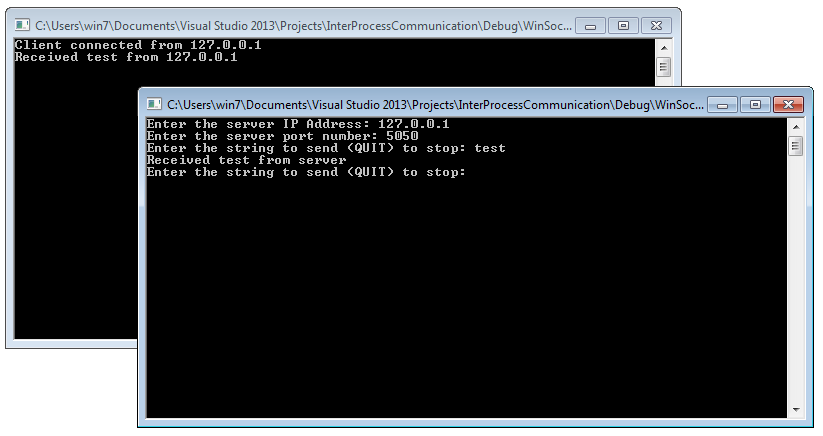
\includegraphics[scale=0.8]{img/06_Winsock}
\caption{Работа с сокетами.}
\end{figure}

\newpage
%------------------------------------------------
\section*{Порты завершения}

Операциям ввода и вывода присуща более медленная скорость выполнения по сравнению с другими видами обработки. Причиной такого замедления являются следующие факторы:

\begin{itemize}
\item Задержки, обусловленные затратами времени на поиск нужных дорожек и секторов на устройствах произвольного доступа (диски, компакт-диски).

\item Задержки, обусловленные сравнительно низкой скоростью обмена данными между физическими устройствами и системной памятью.

\item Задержки при передаче данных по сети с использованием файловых, серверов, хранилищ данных и так далее.
\end{itemize}

Во всех предыдущих примерах операции ввода/вывода выполняются синхронно с потоком, поэтому весь поток вынужден простаивать, пока они не завершатся.

В этом примере показано, каким образом можно организовать продолжение выполнения потока, не дожидаясь завершения операций ввода/вывода, что будет соответствовать выполнению потоками асинхронного ввода/вывода.

Порты завершения оказываются чрезвычайно полезными при построении масштабируемых серверов, способных обеспечивать поддержку большого количества клиентов без создания для каждого из них отдельного потока. 

Листинг 12 показывает реализацию порта завершения. Для работы с ним использовался клиент из предыдущего примера. Визуальной разницы нет, но она драматически ощущается при большом количестве клиентов.

\begin{verbatim}
Листинг 12. Порт завершения.

// http://habrahabr.ru/post/59282/

#include <winsock2.h>
#include <windows.h>
#include <stdio.h>

#pragma comment(lib, "Ws2_32.lib")

//port number to listen
#define SERVER_PORT 7710

enum
{
    SEND_DONE = 0,
    RECV_DONE = 1,
};

typedef struct _USER_DATA
{
    SOCKET sock;
    //more to go
} USER_DATA;

typedef struct _USER_IO
{
    WSAOVERLAPPED ov; //should be first in the struct
    WSABUF buf;
    DWORD optype;
    DWORD flags;
    DWORD bytes;
} USER_IO;

void WorkingThread(HANDLE iocp)
{
    DWORD Bytes;
    USER_DATA * user;
    USER_IO * io;
    while (1)
    {
        if (!GetQueuedCompletionStatus(
            // хендл порта, к пулу которого следует подключиться
            iocp,
            // количество переданных байт
            &Bytes,
            // указатель на ключ завершения
            (PULONG_PTR)&user,
            // указатель на OVERLAPPED, ассоциированную с IO-транзакцией
            (LPOVERLAPPED *)&io,
            // время, на которое поток может уснуть
            INFINITE))
            //error
            break;

        if (!Bytes)
        {
            //descriptor closed
            printf("Disconnected user %d from server.\n", user->sock);
            shutdown(user->sock, SD_BOTH);
            closesocket(user->sock);
            continue;
        }

        switch (io->optype)
        {
        case(SEND_DONE) :
            //just requesting new recv
            WSARecv(user->sock, &io->buf, 1, &io->bytes, &io->flags, &io->ov, 0);
            io->optype = RECV_DONE;
            printf("Welcome to user %d sent.\n", user->sock);
            continue;
        case(RECV_DONE) :
            //    here can be done processing or sheduling
            printf("Got packet from client %d, length %d.\n", user->sock, Bytes);
            WSARecv(user->sock, &io->buf, 1, &io->bytes, &io->flags, &io->ov, 0);
            continue;
        }
    }

    printf("Error %d.\n", GetLastError());
};

int main(int argc, char * argv[])
{
    WSADATA wsadata;
    SOCKADDR_IN listenaddr;
    SOCKET listensocket;
    HANDLE iocp;
    int i;

    WSAStartup(0x0202, &wsadata);

    //making listening socket overlapped
    listensocket = WSASocket(AF_INET, SOCK_STREAM, IPPROTO_TCP,
                                                    0, 0, WSA_FLAG_OVERLAPPED);

    listenaddr.sin_family = AF_INET;
    listenaddr.sin_port = htons(SERVER_PORT);
    listenaddr.sin_addr.S_un.S_addr = INADDR_ANY;

    bind(listensocket, (SOCKADDR *)&listenaddr, sizeof(listenaddr));
    listen(listensocket, 5);

    // создать новый объект порта завершения
    iocp = CreateIoCompletionPort(
        INVALID_HANDLE_VALUE, // аргумент означает новый порт
        0, 0, // всегда 0
        0); // кол-во потоков для порта одновременно (по умолчанию кол-во CPU)
    if (!iocp)
    {
        printf("Can't create IOCP: error %d", GetLastError());
        return 0;
    }

    // Кол-во потоков в пуле
    for (i = 1; i <= 2; ++i)
    {
        HANDLE thr = CreateThread(0, 0,
                (LPTHREAD_START_ROUTINE)&WorkingThread, (LPVOID)iocp, 0, 0);
        CloseHandle(thr);
    }

    // Клиент
    while (1)
    {
        SOCKET clientsocket;
        SOCKADDR clientaddr;
        USER_DATA * user;
        USER_IO * io;
        int clientsize = sizeof(clientaddr);

        user = (USER_DATA *)malloc(sizeof(USER_DATA));
        io = (USER_IO *)malloc(sizeof(USER_IO));
        memset(user, 0, sizeof(USER_DATA));
        memset(io, 0, sizeof(USER_IO));

        // возвращает нам сокет клиента, в который можно писать и читать
        clientsocket = WSAAccept(listensocket,
                                    (SOCKADDR *)&clientaddr, &clientsize, 0, 0);
        printf("Accepted new client %d.\n", clientsocket);

        user->sock = clientsocket;
        io->buf.buf = (char *)malloc(1024);
        strcpy_s(io->buf.buf, 19, "You are connected!");

        io->buf.len = 19;
        io->optype = SEND_DONE;

        // связываем дескрипторы сокета и порта
        CreateIoCompletionPort((HANDLE)clientsocket, iocp, (ULONG_PTR)user, 0);

        //sending welcome message to the client
        WSASend(user->sock, &io->buf, 1, &io->bytes, 0, (LPOVERLAPPED)io, 0);
    }
};
\end{verbatim}

\newpage
%------------------------------------------------
\section*{Сигналы}

В отличии от Linux, сигналы в Windows имеют сильно усеченные возможности. Наиболее сложной задаче при работе с сигналами было придумать, что можно с ними сделать. В листинге 13 по сигналу меняется цвет консоли.

\begin{verbatim}
Листинг 13. Сигналы в Windows.

#include <windows.h>
#include <stdio.h>
#include <iostream>

BOOL CtrlHandler(DWORD fdwCtrlType)
{
    HANDLE hStdout = GetStdHandle(STD_OUTPUT_HANDLE);
    if (hStdout == INVALID_HANDLE_VALUE)
    {
        std::cout << "Error while getting input handle" << std::endl;
        return EXIT_FAILURE;
    }

    switch (fdwCtrlType) //тип сигнала
    {
    // Handle the CTRL-C signal.
    case CTRL_C_EVENT:
        SetConsoleTextAttribute(hStdout, FOREGROUND_RED 
                            | BACKGROUND_BLUE | FOREGROUND_INTENSITY);
        std::cout << "Ctrl-C event\n\n" << std::endl;
        SetConsoleTextAttribute(hStdout, FOREGROUND_RED 
                                | FOREGROUND_GREEN | FOREGROUND_BLUE);
        return(TRUE);
        // CTRL-CLOSE: confirm that the user wants to exit.
    case CTRL_CLOSE_EVENT:
        SetConsoleTextAttribute(hStdout, FOREGROUND_RED
                            | BACKGROUND_BLUE | FOREGROUND_INTENSITY);
        std::cout << "Ctrl-Close event\n\n" << std::endl;
        SetConsoleTextAttribute(hStdout, FOREGROUND_RED
                                | FOREGROUND_GREEN | FOREGROUND_BLUE);
        return(TRUE);
        // Pass other signals to the next handler.
    case CTRL_BREAK_EVENT:
        SetConsoleTextAttribute(hStdout, FOREGROUND_RED
                            | BACKGROUND_BLUE | FOREGROUND_INTENSITY);
        std::cout << "Ctrl-Break event\n\n" << std::endl;
        SetConsoleTextAttribute(hStdout, FOREGROUND_RED 
                                | FOREGROUND_GREEN | FOREGROUND_BLUE);
        return FALSE;
    case CTRL_LOGOFF_EVENT:
        SetConsoleTextAttribute(hStdout, FOREGROUND_RED 
                            | BACKGROUND_BLUE | FOREGROUND_INTENSITY);
        std::cout << "Ctrl-Logoff event\n\n" << std::endl;
        SetConsoleTextAttribute(hStdout, FOREGROUND_RED 
                                | FOREGROUND_GREEN | FOREGROUND_BLUE);
        return FALSE;
    case CTRL_SHUTDOWN_EVENT:
        SetConsoleTextAttribute(hStdout, FOREGROUND_RED 
                            | BACKGROUND_BLUE | FOREGROUND_INTENSITY);
        std::cout << "Ctrl-Shutdown event\n\n" << std::endl;
        SetConsoleTextAttribute(hStdout, FOREGROUND_RED 
                                | FOREGROUND_GREEN | FOREGROUND_BLUE);
        return FALSE;
    default:
        return FALSE;
    }
}
int main(void)
{
    if (SetConsoleCtrlHandler((PHANDLER_ROUTINE)CtrlHandler, TRUE))
    {
        std::cout << "The Control Handler is installed." << std::endl
            << "-- Now try pressing Ctrl+C or Ctrl+Break, or" << std::endl
            << "   try logging off or closing the console..." << std::endl
            << std::endl << "(...waiting in a loop for events...)"
            << std::endl << std::endl;
        while (1){}
    }
    else
    {
        std::cout << "ERROR: Could not set control handler" << std::endl;
        return EXIT_FAILURE;
    }
    return EXIT_SUCCESS;
}
\end{verbatim}

\begin{figure}[h!]
\centering
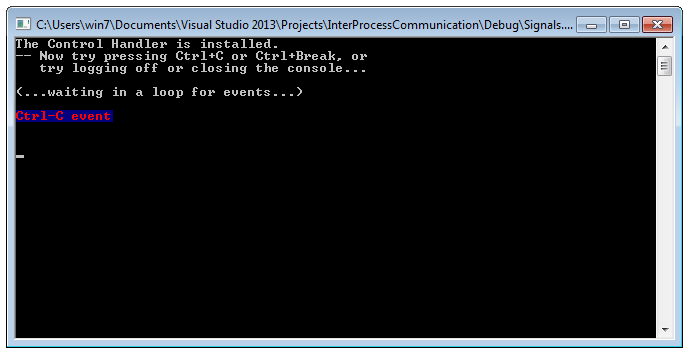
\includegraphics[scale=0.8]{img/07_Signals}
\caption{Работа с сигналами.}
\end{figure}

\newpage
%------------------------------------------------
\section*{Выводы}

В данной работе были рассмотрены основные механизмы межпроцессорного взаимодействия, от самых простых, типа анонимных каналов, до самых сложных, таких как сокеты и порты завершения. Каждый механизм имеет свою нишу для использования.

Отдельно выделяются только сигналы, которые значительно уступают подобному механизму из мира linux.

Наиболее интересным средством взаимодействия оказался сокет. Он не имеет больших отличий от классического сокета Беркли, что упрощает его изучение. Работа в асинхронном режиме (порты завершения) оказывает драматическое влияние на скорость работы системы, и должна применяться в высоко нагруженных системах.

\end{document}
